\chapter{Wyniki}
\label{cha:wyniki}

W tym rozdziale opisana jest metodologia testowania wydajności algorytmów mnożenia macierzy rzadkiej z wektorem dla wartości pojedynczej precyzji (\textit{SpMV}) oraz dokonana jest analiza uzyskanych wyników.

System wykorzystany do przeprowadzenia testów wydajności wyposażony był w procesor graficzny NVIDIA RTX 3060 (GA106) w konfiguracji 130W działający pod sterownikiem w wersji 528.24.
Systemem operacyjnym był Windows 11 w wersji 22H2, kompilator \textit{glslc} \cite{glslcgithub} w wersji v2021.2 oraz VulkanSDK \cite{vulkansdk} w wersji 1.2.182.0.
Na potrzeby testów wykorzystano pięć macierzy: BEAFLW, DENSE2, BCSSTK32, SCIRCUIT i GA41AS41H72.
Każda z nich reprezentuje różne cechy macierzy rzadkich: rozmiar, zagęszczenie, rozpiętość wartości w komórkach i sposób rozmieszczenia elementów.
Każdy algorytm dla danego formatu uruchamiany był 1000 razy, celem zdobycia średniego czasu wykonania danej operacji.

\begin{figure}[!htb]
\minipage{0.45\textwidth}
    \textbf{BEAFLW} ma wymiar $497 \times 507$, z czego $21.193\%$ jest elementami niezerowymi, rozkład przestawiony na rysunku \ref{beaflw_matrix_plot} wykazuje znikome skumulowanie względem przekątnej.
\endminipage\hfill
\minipage{0.45\textwidth}
  \includegraphics[width=\linewidth]{matrix_plots/beaflw.png}
  \caption{Rozkład w macierzy BEAFLW}\label{beaflw_matrix_plot}
\endminipage\hfill
\end{figure}

\pagebreak

\begin{figure}[!htb]
\minipage{0.45\textwidth}
    \textbf{DENSE2} ma wymiar $2000 \times 2000$, z czego $100\%$ elementów ma wartości niezerowe, rozkład przestawiony na rysunku \ref{dense2_plot}.
\endminipage\hfill
\minipage{0.45\textwidth}
  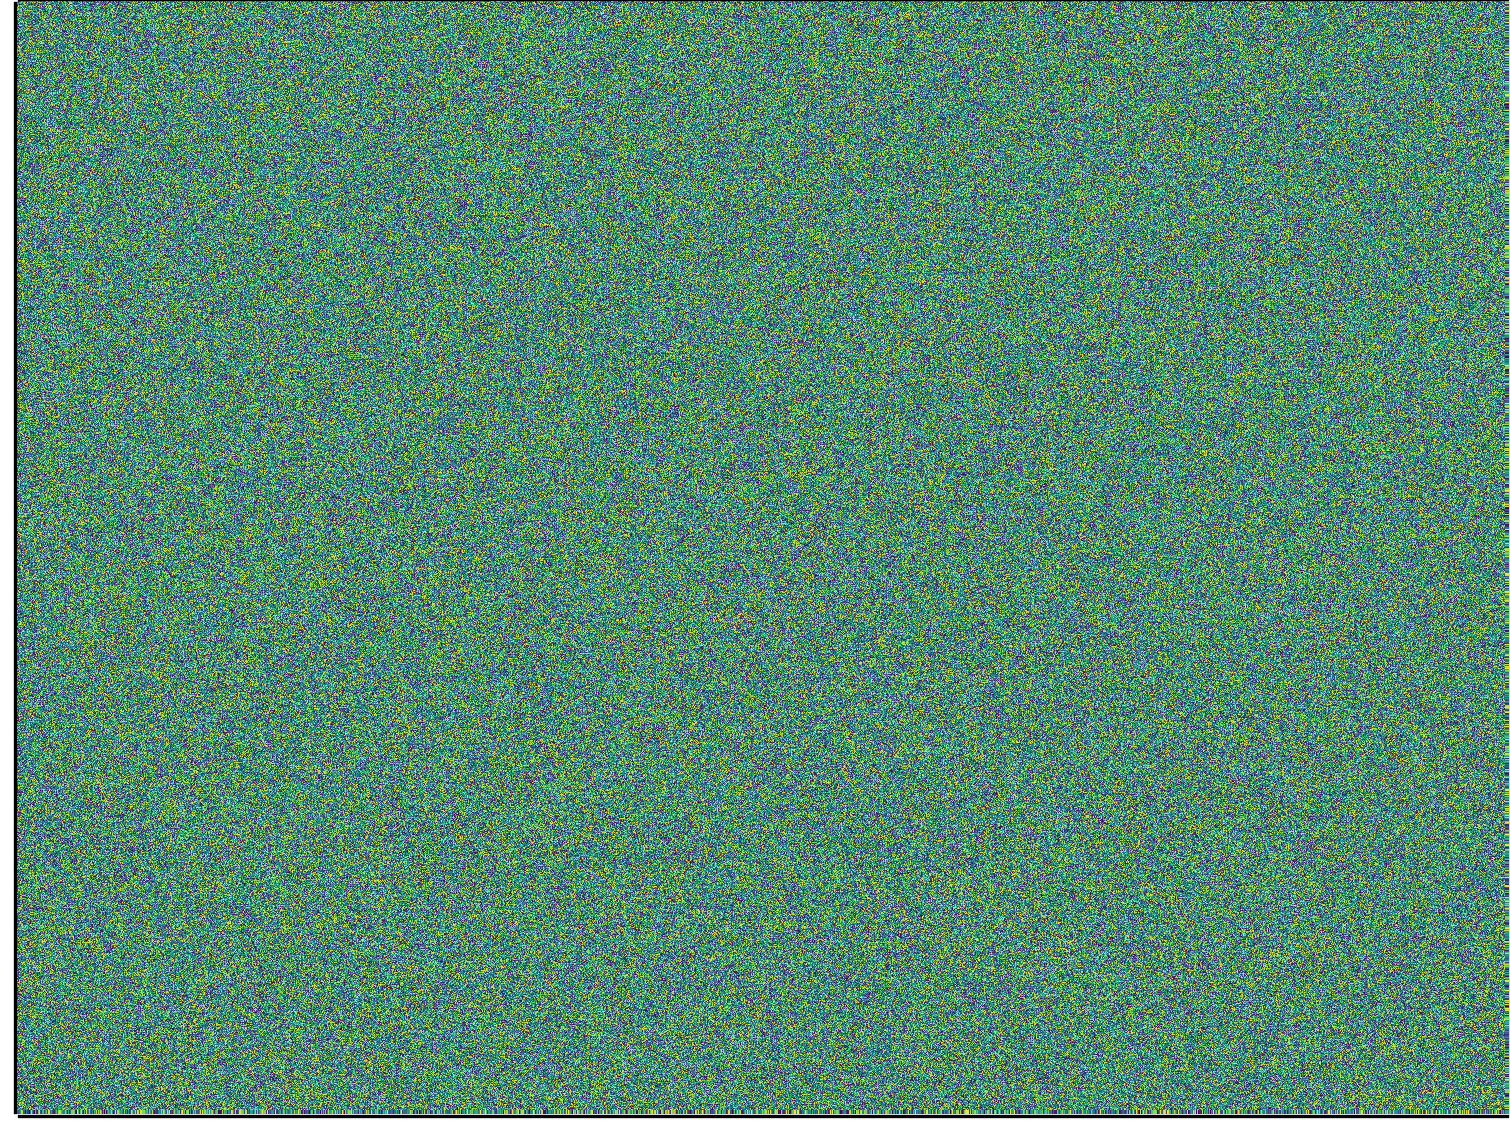
\includegraphics[width=\linewidth]{matrix_plots/dense2.png}
  \caption{Rozkład w macierzy DENSE2}\label{dense2_plot}
\endminipage\hfill
\end{figure}

\begin{figure}[!htb]
\minipage{0.45\textwidth}
    \textbf{BCSSTK32} ma wymiar $44609 \times 44609$, z czego $0.1\%$ jest elementami niezerowymi, rozkład przestawiony na rysunku \ref{bcsstk32_plot} wykazuje symetryczność względem przekątnej i niskie skumulowanie względem niej.
\endminipage\hfill
\minipage{0.45\textwidth}
  \includegraphics[width=\linewidth]{matrix_plots/bcsstk32.png}
  \caption{Rozkład w macierzy BCSSTK32}\label{bcsstk32_plot}
\endminipage\hfill
\end{figure}

\begin{figure}[!htb]
\minipage{0.45\textwidth}
    \textbf{SCIRCUIT} ma wymiar $170998 \times 170998$, z czego $0.003\%$ jest elementami niezerowymi, rozkład przestawiony na rysunku \ref{scircuit_plot} wykazuje symetryczność względem przekątnej i średnie skumulowanie względem niej.
\endminipage\hfill
\minipage{0.45\textwidth}
  \includegraphics[width=\linewidth]{matrix_plots/scircuit.png}
  \caption{Rozkład w macierzy SCIRCUIT}\label{scircuit_plot}
\endminipage\hfill
\end{figure}

\pagebreak

\begin{figure}[!htb]
\minipage{0.45\textwidth}
    \textbf{GA41AS41H72} ma wymiar $268096 \times 268096$, z czego $0.026\%$ jest elementami niezerowymi, rozkład przestawiony na rysunku \ref{ga41as41h72_plot} wykazuje symetryczność względem przekątnej i wysokie skumulowanie względem niej.
\endminipage\hfill
\minipage{0.45\textwidth}
  \includegraphics[width=\linewidth]{matrix_plots/Ga41As41H72.png}
  \caption{Rozkład w macierzy GA41AS41H72}\label{ga41as41h72_plot}
\endminipage\hfill
\end{figure}

Analizując wykres \ref{all_plot} zauważalna jest wysoka wydajność formatu CSR, w dwóch przypadkach jest najwyższa, natomiast w pozostałych jest blisko największej osiągniętej wydajności. 
Format SELL wraz ze zmniejszaniem $C$ osiąga wyższe wyniki zbliżając się wydajnościowo do formatu CSR, co jest oczekiwane, ponieważ dla $C = 1$ format SELL będzie zachowywać się w silnie zbliżony sposób do formatu CSR.
Wydajność formatu ELL nie wyróżniała się ponad inne formaty, pomimo znacznie większego zużycia pamięci.
W ponad połowie przypadków format ten był szybszy niż COO i CSC, natomiast dla macierzy z małym zagęszczeniem lub małą ilością elementów format COO osiągał najwyższą wydajność ze wszystkich formatów.
Pomimo najmniejszego zużycia pamięci format BSR osiągał jedne z najniższych wyników wydajnościowych, im większy rozmiar bloku tym bardziej wydajność spadała.

\begin{figure}[!htb]
    \centering
    \includegraphics[width=\linewidth]{result_plots/barchart.png}
    \caption{Wydajność różnych formatów macierzy}\label{all_plot}
\end{figure}

Wprowadzono pojęcie efektywności formatu, który jest sposobem porównania efektywności wykorzystania pamięci do uzyskania danego poziomu wydajności obliczeniowej, określonego przez stałą $k$:

\begin{equation}
    k = \frac{1}{t \cdot s}
\end{equation}

\begin{eqwhere}[2cm]
	\item[$k$] stała efektywności
	\item[$t$] czas obliczeń
    \item[$s$] rozmiar pamięci potrzebny do reprezentacji macierzy
\end{eqwhere}

Pozwala ona na porównanie w kontekście tej samej macierzy wydajności obliczeniowej w zależności od ilości wykorzystanej pamięci.
Stała ta faworyzuje jak najmniejsze wykorzystanie pamięci i w tym samym momencie jak najszybsze wykonanie programu, format może wykorzystać więcej pamięci jeżeli czas wykonania na tym drastycznie zyskuje.
Porównywanie różnych stałych może zostać dokonane tylko w obrębie tej samej macierzy.
Celem ułatwienia porównań na wykresie \ref{all_k_plot} przedstawiono każdą wartość $k$ przeskalowaną względem stałej $k$ dla formatu CSR.
W skutek tego w każdej macierzy format CSR zyskuje wartość $k = 1$, pozostałe wartości należy interpretować jako mnożnik efektywności tego formatu dla tej macierzy względem formatu CSR.
Wybrano CSR ze względu na średnio najwyższe wyniki oraz stosunkowo niskie zużycie pamięci.
W trzech przypadkach macierzy, format CSR jest najbardziej efektywnym formatem, dla macierzy \textit{DENSE2} jest trochę mniej efektywny niż warianty SELL i dla macierzy \textit{BEAFLW} jest drugi co do efektywności względem formatu COO, która jest 2.5 raza bardziej efektywna.

\begin{figure}[!htb]
    \centering
    \includegraphics[width=\linewidth]{result_plots/barchart_memory.png}
    \caption{Porównanie efektywności wykorzystania pamięci}\label{all_k_plot}
\end{figure}

Finalne wyniki posiadały pewne różnice pomiędzy sobą, największy błąd względny pojedynczego elementu wektora wyjściowego, dla którego bazą był wynik obliczony na jednostce centralnej formatem ELL wynosił $1.894\%$ dla formatu CSC w macierzy GA41AS41H72.
Różnice te są oczekiwanym rezultatem zmiany kolejności wykonywania obliczeń, ponieważ standard IEEE-754  \cite{FloatPoint} nie gwarantuje łączności obliczeń.
Przez to należy rozumieć, iż zachodzi następująca nierówność:

\begin{equation}
    (x+y)+z \neq x+(y+z)
\end{equation}

Połączenie formatu, który rozdziela pracę w przeciwnym kierunku co format ELL oraz atomicznej redukcji do każdego elementu wektora wyjściowego, tworzy środowisko, w którym oczekiwane będzie, iż kolejność wykonywanych operacji będzie różna od tej która miała miejsce podczas obliczeń na jednostce centralnej.
Dodatkowo, duża ilość elementów i niejednolite wartości macierzy GA41AS41H72 tylko potęgują ten efekt. 